\section{\ours: Bootstrapping Tool-Integrated Reasoning via RL for VLMs}
\label{sec:training}

\subsection{Two-Stage Training Framework}
With the developed \env, we enable a two-stage training framework. First, we bootstrap an interactive agent with behavioral cloning (BC), instilling instruction-following and basic tool-use. We then refine it with multi-turn, online RL, which encourages deeper reasoning and disciplined, reasoning-guided tool orchestration.

\noindent \textbf{Stage I: Warmup w. Imitation Learning.}
% To initialize the agent with fundamental instruction-following and tool-use capabilities, we employ behavioral cloning (BC) via supervised fine-tuning (SFT) on synthesized expert trajectories.
% Thus, we construct these trajectories in a structured format to explicitly model both cognitive processes and actions. 
% Ground-truth tool calls are first established by filtering for successful executions across our diverse toolset against verifiable answers. 
% Subsequently, we utilize advanced multimodal models to synthesize the surrounding reasoning traces $g_t$.
% Notably, we prioritize open-source models, like Qwen3-VL family, for trace generation to capture more explicit, extended reasoning chains. 
% The base agent is then trained to maximize the likelihood of these interleaved thought-action sequences using standard cross-entropy loss:
We initialize the policy by BC on synthesized expert trajectories that \emph{explicitly} interleave thoughts and actions. 
(i) \textit{Candidate generation and filtering.} We first generate tool‑executing trajectories with a proprietary model (\texttt{GPT‑5}) and retain only those whose final answers exactly match ground truth (outcome‑based filtering). 
(ii) \textit{Rationale densification.} To strengthen supervision on reasoning, we replace concise rationales with extended traces produced by an open‑weights expert (\texttt{Qwen3‑VL‑235B‑A22B‑Thinking}). 
Let $\mathcal{D}$ denote the resulting set of tuples $(x,\tau)$ where $\tau{=}(g_1,a_1,\ldots,g_T,\hat{y})$ and $c_{t-1}$ is the interaction history up to step $t{-}1$. The BC objective maximizes the likelihood of interleaved thought–action tokens:
% To establish fundamental instruction-following and tool-use capabilities, we initialize the agent via Behavorial Cloning on synthesized expert SFT trajectories. 
% First, we generate candidate trajectories containing tool executions using the proprietary state-of-the-art model, \texttt{GPT-5}, and apply strict outcome-based filtering to discard incorrect solutions.
% To further densify the supervision signal, we enhance the reasonoing quality by leveraging the open-weights expert, \texttt{Qwen3-VL-235B-A22B-Thinking}.
% Specifically, we substitute the initial, concise rationales with the expert's extended reasoning traces for enhanced reasoning capabilities.
% We construct these trajectories by identifying successful tool executions verified against ground-truth answers, then synthesizing the associated reasoning traces $g_t$ using expert multimodal models (e.g., Qwen3-VL) to capture extended thought chains. \wz{Can we be a bit straightforward? This is what I understand: we first use InternVL( or Qwen3VL ?) to generate reasonings, actions, and answers, then filter out the trajectories with incorrect answers. We further augment the reasonings with expert multimodal models (e.g. Qwen3-VL).  }
% The agent is trained to maximize the likelihood of these interleaved thought-action sequences via cross-entropy loss:
\begin{equation*}
    \begin{aligned}
        &\mathcal{L}_{\text{BC}}(\theta)=\mathbb{E}_{(x,\tau)\sim\mathcal{D}}[\log\pi_\theta(\tau|x)]\\
        &=\mathbb{E}\left[\sum_{t=0}^{T-1}\log\pi_\theta(a_t|x,c_{t-1},g_t)+\sum_{t=0}^{T}\log\pi_\theta(g_t|x,c_{t-1})\right].
    \end{aligned}
\end{equation*}
The synthesized corpus covers a diverse tool mix (Figure~\ref{fig:sft-tool-distribution}), providing a robust prior for tool syntax and selection. 

\noindent \textbf{Stage II: Online RL.}
After SFT, we train the agent in the executable environment with multi-turn rollouts, where each step emits a reasoning segment followed by a function call; \env{} executes the call and appends the (structured) feedback to the context for continued reasoning.
For policy improvement, we adopt Group Relative Policy Optimization (GRPO)~\cite{shao2024deepseekmath} with group-normalized advantages over $G$ rollouts:
% Following initial behavioral cloning, we transition to multi-turn online reinforcement learning with the \env environment.
% During the rollout stage, the agent iteratively generates reasoning and tool calls. 
% After each turn, \env provides execution feedback, which is immediately appended to the context to enable continuation of the trajectory.
% For policy optimization, we use the rewards provided by \env and adopt GRPO~\cite{shao2024deepseekmath} to estimate the advantage.
% By computing a relative advantage signal against a group of sampled rollouts, GRPO delivers a strong, low-variance training signal critical for guiding the VLM to learn the explicit reasoning steps and structured action sequences necessary for autonomous tool orchestration.
% Once the model possesses some basic capabilities of reasoning and calling tool functions, we perform the multi-turn online training for our baseline agent in \env{}.
% Specifically in each turn of the rollout stage, we  first prompt the model to generate reasoning and tool calling, and leverage \env{} to provide feedback. We then append the feedback to the generations to continue the generation for the next turn. Along the trajectory,   \env{} also provides rewards, which we shall introduce below, for the policy update.   We adopt  GRPO~\cite{shao2024deepseekmath} to estimate the advantage.
% By computing a relative advantage signal against a group of sampled rollouts, GRPO provides a strong, low-variance training signal that successfully guides the LLM to learn the explicit reasoning steps and action sequences necessary for autonomous tool-call orchestration.
% The objective is given by:
\begin{equation*}
% \setlength{\abovedisplayskip}{3pt}
% \setlength{\belowdisplayskip}{3pt}
    \begin{aligned}
        \mathcal{L}_{\text{GRPO}}(\theta)&=\frac{1}{G}\sum_{i=1}^G\frac{1}{|\tau_i|}\sum_{k=1}^{|\tau_i|}\min[r_{i,k}(\theta)\cdot\hat{A}_{i,k},\\
        &\quad\text{clip}(r_{i,k}(\theta),1-\epsilon,1+\epsilon)\cdot\hat{A}_{i,k}],
    \end{aligned}
\end{equation*}
where $r_{i,k}(\theta)$ denotes the token-level importance ratio at the $k$-th token.
\begin{equation*}
% \setlength{\abovedisplayskip}{3pt}
% \setlength{\belowdisplayskip}{3pt}
    \begin{aligned}
        r_{i,k}(\theta)&=\frac{\pi_\theta(\tau_{i,k}|\tau_{i,<k})}{\pi_{\text{old}}(\tau_{i,k}|\tau_{i,<k})},
    \end{aligned}
\end{equation*}
and $\hat{A}_{i,k}$ is the normalized advantage across all tokens:
\begin{equation*}
    \begin{aligned}
        \quad \hat{A}_{i,k}&=\frac{R(\tau_i)-\text{mean}(\{R(\tau_1),\cdots,R(\tau_G)\}}{\text{std}(\{R(\tau_1),\cdots,R(\tau_G)\})}.
    \end{aligned}
\end{equation*}

% \subsection{Tool-Use Additional Design} 
% mask out tool observation tokens (follow SimpleTIR)
% (1) intermediate stop with tool call detected
% (2) mask out tool feedback when appending back to the generation
% \yz{@lumeng, check}
% % effiiency

% \yz{@lumeng, add tool set selection criteria/motivation and tool description here}

% \yz{maybe we need to add some visualization here. VAGEN figure 3 is good.}

% \noindent \textbf{Domain-Specific VLMs as Tools.}
% Among the aforementioned selected tools, G-LLaVA~\cite{gao2025gllava} and ChartMoE~\cite{xu2025chartmoe} are heavy-weight VLMs as interactive tools, and require significant amount of computational resource.
% To address the issue and integrate them into our distributed RL framework, we developed a highly concurrent microservices architecture. 
% Unlike traditional monolithic setups, our system decouples model inference from the primary training loop, deploying each VLM as an independent HTTP service.
% This architecture is built on a three-tier design: 
% (1) a \textbf{FastAPI} top layer that provides RESTful interfaces for asynchronous request batching;
% (2) an intermediate \textbf{Tool} layer responsible for parsing instruction actions, extracting image data from trajectory metadata, and formatting observations;
% and (3) a foundational \textbf{Ray Actor} layer, which maintains model parameters persistently in GPU memory upon initialization, eliminating the prohibitive latency overhead of repetitive model reloading during high-frequency tool calls.

% \noindent \textbf{Asynchronous Training.}
% Achieving high throughput is critical for efficient large-scale RL training. 
% We leverage the Ray distributed framework to manage concurrency, enabling the system to handle massive parallel requests generated by the model.
% For each rollout, the model will need to first generate a reasoning piece, embraced with \texttt{<think>} and \texttt{</think>}, and then generate a function call also embraced in \texttt{<tool\_call>} and \texttt{</tool\_call>}.
% When detecting the special token \texttt{</tool\_call>}, the model stop generation and the training framework packages the instruction alongside trajectory identifiers and image paths into batched HTTP requests. 
% These requests are asynchronously dispatched to the appropriate tool servers where Ray automatically manages task queues and load balancing across configured GPU resources.
% Furthermore, our system also supports fine-grained resource control, binding intensive VLM toosl to specific GPU devices while allowing lightweight CPU tools to share resources to ensure maximal hardware utilization without overloading.

% \noindent \textbf{Flexible Tool Set.}
% To enable flexible and extensible tool-use capabilities for tasks that may not be covered in the experiments, the system is also designed for robustness and ease of extension.
% We introduce a generic \texttt{BaseTool} class, allowing new tools to be integrated via a standardized interface, which can rapidly expand the VLM agent's capabilities.
% Operational stability is maintained through comprehensive monitoring endpoints (\texttt{/health}, \texttt{/metrics}) and Ray’s automated failure recovery, which restarts crashed actors without disrupting the broader training process. 
% This design effectively transforms diverse, standalone VLMs into highly available, concurrent microservices, seamlessly supporting the intense computational demands of distributed RL training.

\subsection{Reward Design}
% Our reward function $R$ is crafted to enforce a strict, multi-level interaction protocol, evolving from a nascent binary validation rule into a diagnosable, hierarchical structure. 
% The code objective is to incentivize adherence to a predefined ``two-round interaction protocol'', which indicates the required generation structure for tool-use and final answering.
% We define the agent's generation at turn $i$ as $u_i$, and the entire $T$-turn generation as $U=(u_0,u_1,\cdots,u_{T})$.
% The protocol mandates the specific structural format for each turn:
% (1) \textbf{Turn ($<T$) (Tool Call):} the first turns $u_{i<T}$ should generate reasoning with function calls: $u_{i<T}=\text{<think>}\cdots\text{</think>}\text{<tool\_call>}\cdots\text{</tool\_call>}$; 
% (2) \textbf{Turn $T$ (Final Answer):} the last turn $u_T$ should generate reasoning with final answer: $u_T=\text{<think>}\cdots\text{</think>}\text{<answer>}\cdots\text{</answer>}$.
% , where the first turns $u_{i<T}$ should generate reasoning with function calls, while the last turn should be reasoning with final answer:
% \begin{equation*}
%     \begin{aligned}
%     \left\{
%     \begin{aligned}
%         u_{i<T}&=\text{<think>}\cdots\text{</think>}\text{<tool\_call>}\cdots\text{</tool\_call>}\\
%         u_T&=\text{<think>}\cdots\text{</think>}\text{<answer>}\cdots\text{</answer>}
%     \end{aligned}
%     \right.
%     \end{aligned}
% \end{equation*}
We employ a multi-round interaction protocol, $U=(u_0,u_1,\cdots,u_{T})$, for agent training, and design the following rewards $R$ for policy update. This protocol mandates the structural format for each turn $u_i$, enforcing an explicit \textit{think}$\rightarrow$\textit{tool\_call} loop prior to a \textit{think}$\rightarrow$\textit{answer} termination:

\noindent~$\bullet$ \textbf{Turn ($<T$) (Tool Call):} the first turns $u_{i<T}$ should generate reasoning with function calls: 
% $u_{i<T}=\text{<think>}\cdots\text{</think>}\text{<tool\_call>}\cdots\text{</tool\_call>}$;
\begin{equation*}
    \begin{aligned} u_{i<T}=\text{<think>}\cdots\text{</think>}\text{<tool\_call>}\cdots\text{</tool\_call>}.
    \end{aligned}
\end{equation*}

\noindent~$\bullet$ \textbf{Turn $T$ (Final Answer):} the last turn $u_T$ should generate reasoning with final answer:
\begin{equation*}
    \begin{aligned}
u_T=\text{<think>}\cdots\text{</think>}\text{<answer>}\cdots\text{</answer>}.
    \end{aligned}
\end{equation*}
% \begin{itemize}
%     \item \textbf{Turn ($<T$) (Tool Call):} the first turns $u_{i<T}$ should generate reasoning with function calls:
%     \begin{equation*}
%         \begin{aligned}
%             u_{i<T}=\text{<think>}\cdots\text{</think>}\text{<tool\_call>}\cdots\text{</tool\_call>}
%         \end{aligned}
%     \end{equation*}
%     \item \textbf{Turn $T$ (Final Answer):} the last turn $u_T$ should generate reasoning with final answer:
%     \begin{equation*}
%         \begin{aligned}
%             u_T=\text{<think>}\cdots\text{</think>}\text{<answer>}\cdots\text{</answer>}
%         \end{aligned}
%     \end{equation*}
% \end{itemize}


\noindent\textbf{Repetition Penalty.}
We first apply a high‑priority repetition detector $R_{\text{rep}}(U)\!\in\!\{-3.0,-2.0,-1.5,0\}$ that scans for contiguous token/phrase/character repeats and assigns a severity‑dependent negative reward (extreme, severe, moderate, none). This term dominates all subsequent logic. 

% To evaluate this, we first define a high-priority continuous repetition detection function, $R_{\text{rep}}(U)$, which identifies contiguous token, phrase, or character repetitions and returns a potent negative reward based on severity, overriding all other logic.
% Thus, we set a 4-level fine-grained reward penalty: $-3.0$ for extreme, $-2.0$ for severe, $-1.5$ for moderate, and $0$ for no repetition.
% \begin{equation*}
%     \begin{aligned}
%         R_{\text{rep}}(U)=\left\{
%         \begin{aligned}
%             &-3.0, & \text{if repetition is extreme},\\
%             &-2.0, & \text{if repetition is severe}, \\
%             &-1.5, & \text{if repetition is moderate}, \\
%             &0.0, & \text{otherwise}.
%         \end{aligned}
%         \right.
%     \end{aligned}
% \end{equation*}

\noindent\textbf{Format Reward.}
Conditional on \emph{no} repetition, $R_{\text{rep}}(U){=}0$, we validate structural well‑formedness (\eg, correct tags, order, and non‑nested closure) at every turn. We define:
% This gating ensures structure is rewarded/penalized only when repetition is absent. Specifically, we define:
\begin{equation*}
% \setlength{\abovedisplayskip}{5pt}
% \setlength{\belowdisplayskip}{5pt}
    \begin{aligned}
        R_{\text{format}}(U)=(\mathbb{I}\{\text{all $u_i$ conforms the format}\}-0.5)\times2.
        % \left\{
        % \begin{aligned}
        %     &+1.0, &\text{if all $u_i$ conforms the format},\\
        %     &-1.0, &\text{otherwise}.
        % \end{aligned}
        % \right.
    \end{aligned}
\end{equation*}



% If, and only if, $R_\text{rep}(U)=0$, we proceed to the structural validation function $R_{\text{format}}(U)$, which acts as a format reward function, verifying that the generation $u_i$ perfectly matches the required pattern for $i$-th turn, ensuring correct tag presence, order, and non-nested closure.
% Any deviation (e.g., missing tags, incorrect ordering, or malformed structure) results in a penalty.
% \begin{equation*}
%     \begin{aligned}
%         R_{\text{format}}(U)=(\mathbb{I}\{\text{all $u_i$ conforms the format}\}-0.5)\times2.
%         % \left\{
%         % \begin{aligned}
%         %     &+1.0, &\text{if all $u_i$ conforms the format},\\
%         %     &-1.0, &\text{otherwise}.
%         % \end{aligned}
%         % \right.
%     \end{aligned}
% \end{equation*}

\noindent\textbf{Correctness Reward.}
We extract the final prediction $\hat{y}$ from \texttt{<answer>}…\texttt{</answer>} for rule‑based checking. To keep the signal low‑noise and format‑aware, correctness is credited only for repetition‑free, well‑formed outputs:
% The model is required to put the final direct answer or option in the \texttt{<answer>} and \texttt{</answer>}, enabling reliable rule-based verification of correctness. 
% If the extracted answer $\hat{y}$ from the last turn generation $u_{T}$ matches the ground truth $y$, the correctness reward will be $1.0$, otherwise it will be $0.0$: $R_{\text{correct}}(U)=\mathbb{I}\{\hat{y}=y\}$.
\begin{equation*}
% \setlength{\abovedisplayskip}{5pt}
% \setlength{\belowdisplayskip}{5pt}
    \begin{aligned}
        R_{\text{correct}}(U)=\mathbb{I}\{\hat{y}=y\}.
    \end{aligned}
\end{equation*}

\noindent\textbf{Final Reward.}
The rollout‑level reward is the sum of the three components:
\begin{equation*}
% \setlength{\abovedisplayskip}{5pt}
% \setlength{\belowdisplayskip}{5pt}
    \begin{aligned}
        R(U)=R_{\text{rep}}(U)+R_{\text{format}}(U)+R_{\text{correct}}(U).
    \end{aligned}
\end{equation*}
This sparse, format‑aware design allocates positive reward only to generations that are repetition‑free, structurally valid, and correct, thereby encouraging the policy to internalize the intended \textit{think}$\rightarrow$\textit{tool\_call}$\rightarrow$\textit{answer} protocol rather than exploiting intermediate heuristics.  
% This sparse reward design allocates positive feedback only to structurally valid generations free from anomalies (e.g., repetition). This compels the model to internalize the explicit interaction logic—reasoning combined with tool invocation—rather than solely optimizing for task completion, fostering stable and interpretable generative policies.

\begin{figure}
    \centering
    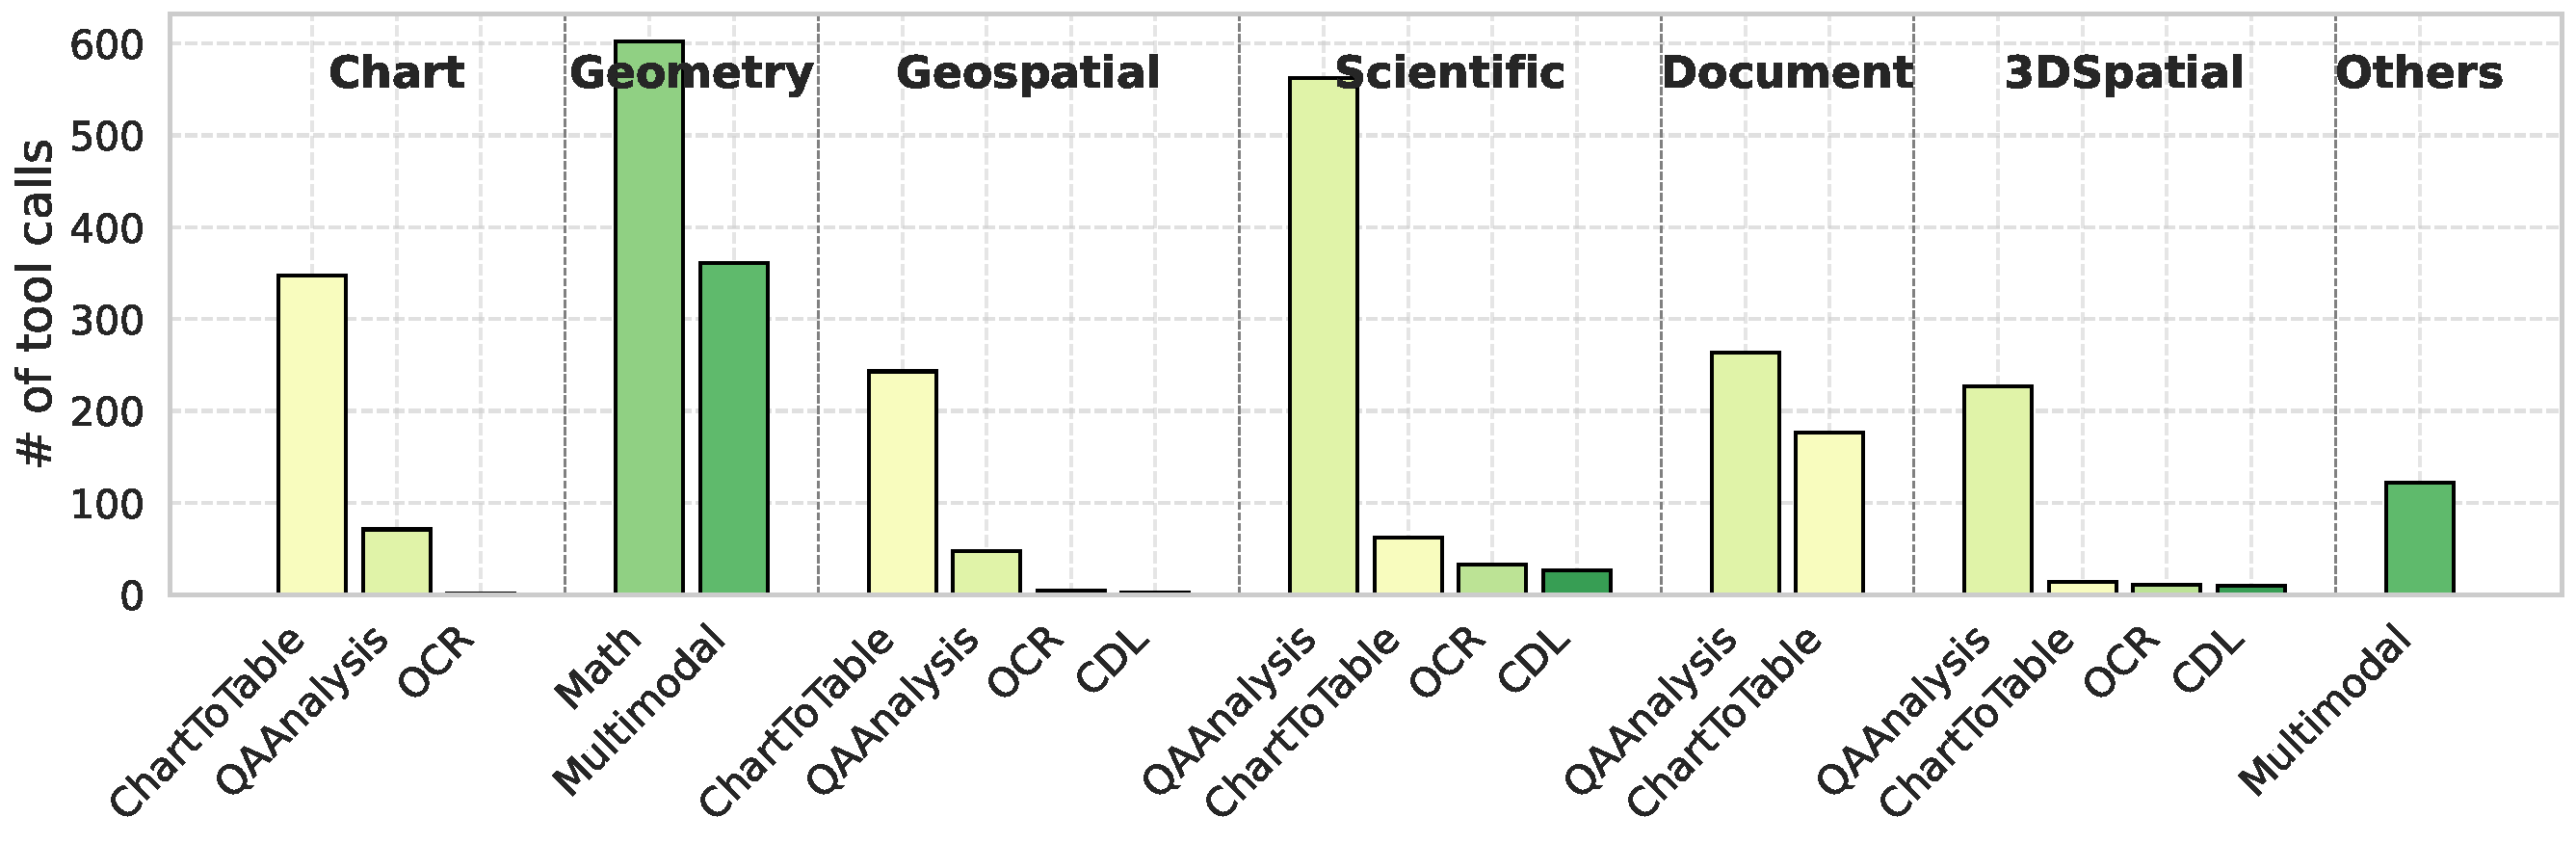
\includegraphics[width=\linewidth]{figure/tool-distribution.pdf}
    % \vspace{-1ex}
    \caption{Top tool call distribution of different tasks in SFT data.}
    % \vspace{-1ex}
    \label{fig:sft-tool-distribution}
\end{figure}
